% !TEX root = ../main.tex

\setcounter{chapter}{-1}

\chapter{Template Instructions}
\label{ch:template-instructions}

Read the README before you start here. Then take a look at the below examples, both in the PDF and in the source code, to get an idea of how to use this template. Delete this chapter before your final submission.

\section{Chapters and Sections}
\label{sec:chapters-and-sections}

You can begin new chapters and sections with the \texttt{\textbackslash chapter} and \texttt{\textbackslash section} commands. This goes down over \texttt{\textbackslash subsection} to the \texttt{\textbackslash subsubsection} level.

Do not skip any of the section levels and always include at least one sentence between successive headings. Also, use title case consistently for all headings. If you are unsure, consult the Title Case Converter at \url{https://titlecaseconverter.com}.

\section{Acronyms}
\label{sec:acronyms}

Acronyms can be included with the \texttt{\textbackslash ac} command and are fully written out on first use, for example \ac{rwth}. On subsequent uses, only the short version is inserted, like \ac{rwth}.

For plural versions, use \texttt{\textbackslash acp}, giving \acp{rwth}. If you want to force the long or short version anywhere, use \texttt{\textbackslash acl} or \texttt{\textbackslash acs}. Don't use acronym commands in chapter or section titles.

Do not use the acronym commands inside \texttt{\textbackslash chapter} or \texttt{\textbackslash section} commands! This breaks compilation when the headings are cross-referenced with \texttt{\textbackslash cref}. Just write the acronym or long version out in plain text.

\section{Citations}
\label{sec:citations}

Use the \texttt{\textbackslash cite} command to insert citations, like~\cite{sutton_reinforcement_2018}. Multiple citations can be added with comma separation in a single command. It is recommended to include a non-breaking space before the citation with \texttt{\textasciitilde}.

To insert the authors~\citeauthor{sutton_reinforcement_2018} or year~\citeyear{sutton_reinforcement_2018} use \texttt{\textbackslash citeauthor} and \texttt{\textbackslash citeyear}. With \texttt{\textbackslash textcite} you can insert a combined author and number citation like \textcite{sutton_reinforcement_2018}.

\section{Cross-References}
\label{sec:cross-references}

Insert cross-references to other sections, figures, equations, etc. with the \texttt{\textbackslash cref} command. This includes not only the number but also the text part, for example \cref{sec:chapters-and-sections}, \cref{fig:label}, \cref{tab:label}, \cref{eq:label}, \cref{list:label2} or \cref{alg:label}.

Multiple references can be added with comma separation (without spaces) in a single \texttt{\textbackslash cref} command, like \cref{fig:label,fig:agent-environment}.

\section{SI Units}
\label{sec:si-units}

Use \texttt{\textbackslash num} and \texttt{\textbackslash qty} commands for pretty printing of numbers and units. For example, large numbers like \num{42000}, percentages like \qty{20}{\percent}, or ranges like \qtyrange{1.5}{2.5}{\meter\per\second} and lists like \qtylist{1.3;6.7;8.0}{\milli\meter}.

\section{TODO Notes}
\label{sec:todo-notes}

You can add remarks\TODO{This is a remark} in the page margin with the \texttt{\textbackslash TODO} command. Inline remarks are also possible, see below, or you can hide the line.
\TODO[inline]{This is an inline remark}

An overview of all remarks\TODO[noline]{Another remark} is printed in the list of TODOs at the end of the document. The remarks and the list disappear if you add the \texttt{final} option to the \texttt{\textbackslash documentclass} command in the preamble.

\section{Equations}
\label{equations}

This template is set up to replace \texttt{(}, \texttt{)}, \texttt{[}, and \texttt{]} in math mode with \texttt{\textbackslash left(}, \texttt{\textbackslash right)}, \texttt{\textbackslash left[}, and \texttt{\textbackslash right]}. This means you don't have to worry about parentheses and bracket size adjustments. Just use them naturally like
\begin{equation}
  \label{eq:label}
  (1 - a) \cdot (1 - \frac{b}{c})
  \text{.}
\end{equation}

For bold symbols, use the \texttt{\textbackslash symbf} command that works for both Latin and Greek letters like $\symbf{x}$ and $\symbf{\phi}$ (as opposed to \texttt{\textbackslash mathbf}). It also fixes some alignment issues, e.g. $\tilde{\symbf{A}}$ versus $\tilde{\mathbf{A}}$. Similarly, you can use \texttt{\textbackslash symcal} or \texttt{\textbackslash symbb} and other commands instead of their \texttt{\textbackslash math\dots} counterparts.

Keep in mind that equations are part of the sentence, so punctuation like full stops and commas still need to be inserted after equations like this geometric series
\begin{equation}
  \label{eq:label2}
  \sum_{k=0}^\infty q^k = \frac{1}{1-q}
  \quad\text{with}\quad
  \abs{q} < 1
  \text{.}
\end{equation}

For proofs, use the \texttt{\textbackslash begin\{proof\} \dots\ \textbackslash end\{proof\}} environment. This can be combined with the \texttt{\textbackslash begin\{theorem\} \dots\ \textbackslash end\{theorem\}} environment if applicable.

\begin{theorem}[Even Squares]
  For all integers $n$, if $n$ is even, then the square of $n$ is even.
\end{theorem}

\begin{proof}
  Let $n$ be any even integer. Then $n = 2k$ for some integer $k$ and
  $$n^2 = (2k)^2 = 4k^2 = 2(2k^2) \text{.}$$
  Since $2k^2$ is an integer, $n^2$ is even.
\end{proof}

\section{Listings}
\label{sec:listings}

Source code listings can be included from files with the \texttt{\textbackslash lstinputlisting} command or directly inside \texttt{lstlisting} environments. You can specify captions and labels as well. Additionally specify the language for basic syntax highlighting.

\lstinputlisting[caption={Caption.},label={list:label},language=c++]
  {listings/hello-world.cpp}

\begin{lstlisting}[caption={Caption.},label={list:label2},language=python]
print("Hello World!")  # comment
\end{lstlisting}

\section{Floating Elements}
\label{sec:floating-elements}

Figures, tables and algorithms are floating elements in \TeX. Here are some examples, mostly just to be referenced from \cref{sec:cross-references}.

\begin{figure}[!ht]
  \centering
  
\includegraphics[width=0.66\textwidth]{template-instructions/agent-environment}
  \caption{The agent-environment interaction in a \ac{mdp}, adapted from \textcite{sutton_reinforcement_2018}. In each time step, the agent observes a state~$S^t$ and a reward~$R^t$ and chooses an action~$A^t$. This leads to a change in the environment and a new state~$S^{t+1}$ and reward~$R^{t+1}$ are issued.}
  \label{fig:agent-environment}
\end{figure}

\begin{figure}[!ht]
  \centering
  \begin{subfigure}[b]{0.32\textwidth}
    \centering
    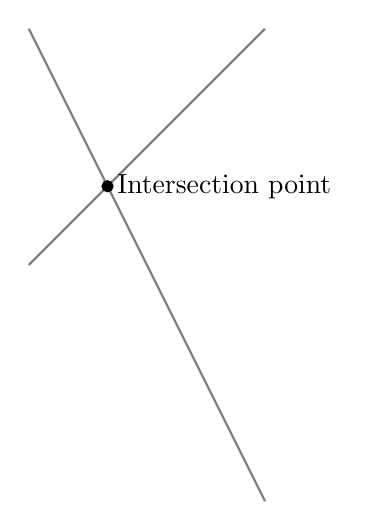
\begin{tikzpicture}
      \draw[gray, thick] (-1,2) -- (2,-4);
      \draw[gray, thick] (-1,-1) -- (2,2);
      \filldraw[black] (0,0) circle (2pt) node[anchor=west]{Intersection point};
    \end{tikzpicture}
    \caption{Caption A}
    \label{fig:label_a}
  \end{subfigure}
  \hfill
  \begin{subfigure}[b]{0.66\textwidth}
    \centering
    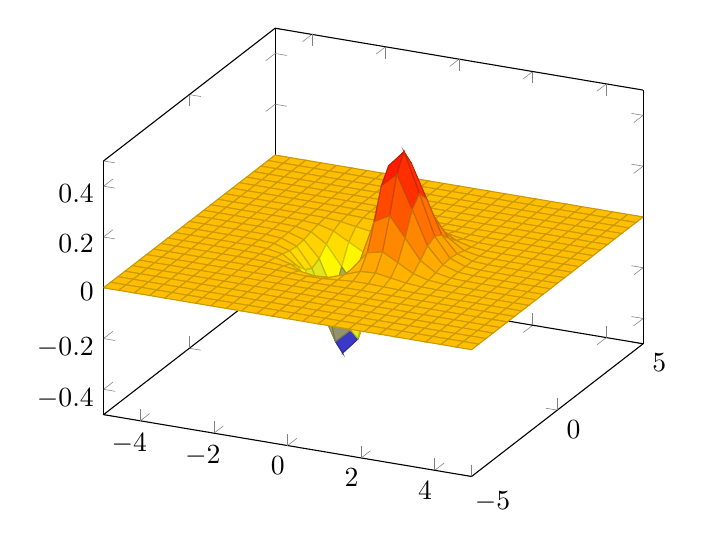
\begin{tikzpicture}
  \begin{axis}
  \addplot3[surf,]
  {exp(-x^2-y^2)*x};
  \end{axis}
\end{tikzpicture}
    \caption{Caption B}
    \label{fig:label_b}
  \end{subfigure}
  \caption{Caption.}
  \label{fig:label}
\end{figure}

\begin{figure}[!ht]
  \centering
  \begin{subfigure}[b]{0.32\textwidth}
    \centering
    \includegraphics[width=\textwidth]{example-image-a}
    \caption{Caption A}
    \label{fig:label_a2}
  \end{subfigure}
  \hfill
  \begin{subfigure}[b]{0.32\textwidth}
    \centering
    \includegraphics[width=\textwidth]{example-image-b}
    \caption{Caption B}
    \label{fig:label_b2}
  \end{subfigure}
  \hfill
  \begin{subfigure}[b]{0.32\textwidth}
    \centering
    \includegraphics[width=\textwidth]{example-image-c}
    \caption{Caption C}
    \label{fig:label_c2}
  \end{subfigure}
  \caption{Caption.}
  \label{fig:label2}
\end{figure}

\begin{table}[!ht]
  \small
  \centering
  \caption{Caption.}
  \label{tab:label}
  \begin{tabularx}{\textwidth}{X | c S[table-format=2.1]}
    \toprule
    \textbf{Column A} & \textbf{Column B} & {\textbf{Column C}} \\
    \midrule
    Row 1 & Text & 42.0 \\
    Row 2 & Text & 31.4 \\
    \bottomrule
  \end{tabularx}
\end{table}

\begin{table}[!ht]
  \small
  \centering
  \caption{Caption.}
  \label{tab:label2}
  \begin{tabular}{l | c S[table-format=2.1]}
    \toprule
    \textbf{Column A} & \textbf{Column B} & {\textbf{Column C}} \\
    \midrule
    Row 1 & Text & 42.0 \\
    Row 2 & Text & 31.4 \\
    \bottomrule
  \end{tabular}
\end{table}

\begin{algorithm}[!ht]
  \caption{Greatest common denominator.}
  \label{alg:label}
  \begin{algorithmic}[1]
  \Procedure{Euclid}{$a,b$} \Comment{Finds the g.c.d. of $a$ and $b$}
    \State $r \gets a \bmod b$
    \While{$r \ne 0$} \Comment{We have a result if $r=0$}
      \State $a \gets b$
      \State $b \gets r$
      \State $r \gets a \bmod b$
    \EndWhile
    \State \Return $b$ \Comment{The g.c.d. is b}
  \EndProcedure
  \end{algorithmic}
\end{algorithm}
